\documentclass[12pt]{article}
\usepackage[paper=letterpaper,margin=1.5cm]{geometry}
\usepackage{amsmath}
\usepackage{amssymb}
\usepackage{amsfonts}
\usepackage{mathtools}
%\usepackage[utf8]{inputenc}
%\usepackage{newtxtext, newtxmath}
\usepackage{lmodern}     % set math font to Latin modern math
\usepackage[T1]{fontenc}
\renewcommand\rmdefault{ptm}
%\usepackage{enumitem}
\usepackage[shortlabels]{enumitem}
\usepackage{titling}
\usepackage{graphicx}
\usepackage[colorlinks=true]{hyperref}
\usepackage{setspace}
\usepackage{subfigure} 
\usepackage{braket}
\usepackage{color}
\usepackage{tabularx}
\usepackage[table]{xcolor}
\usepackage{listings}
\usepackage{mathrsfs}
\usepackage{stackengine}
\usepackage{physics}
\usepackage{afterpage}
\usepackage{pdfpages}
\usepackage[export]{adjustbox}
\usepackage{biblatex}

\setstackEOL{\\}

\definecolor{dkgreen}{rgb}{0,0.6,0}
\definecolor{gray}{rgb}{0.5,0.5,0.5}
\definecolor{mauve}{rgb}{0.58,0,0.82}


\lstset{frame=tb,
  language=Python,
  aboveskip=3mm,
  belowskip=3mm,
  showstringspaces=false,
  columns=flexible,
  basicstyle={\small\ttfamily},
  numbers=none,
  numberstyle=\tiny\color{gray},
  keywordstyle=\color{blue},
  commentstyle=\color{dkgreen},
  stringstyle=\color{mauve},
  breaklines=true,
  breakatwhitespace=true,
  tabsize=3
}
\setlength{\droptitle}{-6em}

\makeatletter
% we use \prefix@<level> only if it is defined
\renewcommand{\@seccntformat}[1]{%
  \ifcsname prefix@#1\endcsname
    \csname prefix@#1\endcsname
  \else
    \csname the#1\endcsname\quad
  \fi}
% define \prefix@section
\newcommand\prefix@section{}
\newcommand{\prefix@subsection}{}
\newcommand{\prefix@subsubsection}{}
\renewcommand{\thesubsection}{\arabic{subsection}}
\makeatother
\DeclareMathOperator*{\argmin}{argmin}
\newcommand{\partbreak}{\begin{center}\rule{17.5cm}{2pt}\end{center}}
\newcommand{\alignbreak}{\begin{center}\rule{15cm}{1pt}\end{center}}
\newcommand{\tightalignbreak}{\vspace{-5mm}\alignbreak\vspace{-5mm}}
\newcommand{\hop}{\vspace{1mm}}
\newcommand{\jump}{\vspace{5mm}}
\newcommand{\R}{\mathbb{R}}
\newcommand{\C}{\mathbb{C}}
\newcommand{\N}{\mathbb{N}}
\newcommand{\G}{\mathbb{G}}
\renewcommand{\S}{\mathbb{S}}
\newcommand{\bt}{\textbf}
\newcommand{\xdot}{\dot{x}}
\renewcommand{\star}{^{*}}
\newcommand{\ydot}{\dot{y}}
\newcommand{\lm}{\mathrm{\lambda}}
\renewcommand{\th}{\theta}
\newcommand{\id}{\mathbb{I}}
\newcommand{\si}{\Sigma}
\newcommand{\Si}{\si}
\newcommand{\inv}{^{-1}}
\newcommand{\T}{^\intercal}
\renewcommand{\tr}{\text{tr}}
\newcommand{\ep}{\varepsilon}
\newcommand{\ph}{\varphi}
%\renewcomand{\norm}[1]{\left\lVert#1\right\rVert}
\definecolor{cit}{rgb}{0.05,0.2,0.45}
\addtolength{\jot}{1em}
\newcommand{\solution}[1]{

\noindent{\color{cit}\textbf{Solution:} #1}}

\newcounter{tmpctr}
\newcommand\fancyRoman[1]{%
  \setcounter{tmpctr}{#1}%
  \setbox0=\hbox{\kern0.3pt\textsf{\Roman{tmpctr}}}%
  \setstackgap{S}{-.9pt}%
  \Shortstack{\rule{\dimexpr\wd0+.1ex}{.9pt}\\\copy0\\
              \rule{\dimexpr\wd0+.1ex}{.9pt}}%
}

\newcommand{\Id}{\fancyRoman{2}}

% Enter the specific assignment number and topic of that assignment below, and replace "Your Name" with your actual name.
\title{STAT 31020: Homework 5}
\author{Caleb Derrickson}
\date{February 14, 2024}

\begin{document}
\onehalfspacing
\maketitle
\allowdisplaybreaks

\tableofcontents

\newcommand{\scI}{\mathcal{I}}
\newcommand{\scE}{\mathcal{E}}
\newcommand{\scA}{\mathcal{A}}
\newcommand{\scL}{\mathcal{L}}
\newcommand{\scF}{\mathcal{F}}
\renewcommand{\grad}{\nabla}

\newpage
\section{Problem 1}
We will aim to prove the first-order optimality conditions Theorem 12.1 and a slightly weaker version of the second-order optimality conditions Theorem 12.5 by assuming the ones for constrained optimization. That is: we will aim to solve the problem (which I will call the ORIGINAL problem) 
\begin{align}
    &\min_{x \in \R^n} f(x)\label{original}\\ &\text{s.t} \quad c_i(x) = 0, \ i \in \scE \nonumber\\
    &\hspace{8mm} c_i(x) \geq 0, \ i \in \scI\nonumber
\end{align}
where the functions $f, c_i$ are smooth (three times continuously differentiable is sufficient, that is what we will assume here), and $ \scI, \scE$ are two indices of sets (typically 1:m, m+1:m+p, but the set notation is much more convenient). A point which only satisfies the constraints is called \textit{feasible}. At such a point some of the inequality constraints may be satisfied with equality, they are said to be \textit{active}. We will denote by the active set at a feasible point x, $\scA (x) = \{ i \in \scE \cup \scI : c_i(x) = 0\}$. observe that $\scE \subset \scA(x)$. \par

\hop
We aim to characterize the properties of a local minimum $x\star$, an extension of the first-order and second-order optimality conditions of unconstrained minimization. An important quantity used to express these conditions is the Lagrangian
\begin{align}
    \scL (x, \lm) = f(x) - \sum_{i \in \scE \cup \scI} \lm_i c_i(x). \label{lagrangian}
\end{align}
Here $\lm_i$ are called the Lagrange multipliers. We will assume that at the solution $x\star$ we satisfy the linear independence constraint qualification (LICQ). That is, we assume the at the set of vectors $\grad_i c_i(x\star), \ i \in \scA(x\star)$ is linearly independent. I call the matrix $J$, whose rows are these vectors, the Jacobian (compare with 12,37 that defines the same quantity). Therefore, we will assume $J$ to be full row rank. Observe one standard awkwardness optimization notation standard: gradients of individual functions are thought of as columns but if you look at the definition of the Jacobian they are thought of as rows.  

\newpage
\subsection{Problem 1, part 1}
Read theorem 12.1 and 12.5 and specialize them for the case of equality constraints only. In particular observe that the critical cone and tangent cone coincide in this case (when it comes to interpreting 12.5).
\partbreak
\begin{solution}

    When transforming Theorem 12.1 and Theorem 12.5 into the desired form, we can assume $\scI = \phi$, that is, the empty set. Therefore, $i \in \scE \cup \scI = \scE$. Thus, when writing Theorem 12.1, which I will call the KKT conditions, we have the following:
    \begin{align*}
        \hspace{40mm}\grad_x \scL (x\star, \lm\star) &= 0,\\
        c_i(x\star) &= 0, \quad \text{for all } i \in \scE,\\
        \lm_i\star c_i(x\star) &= 0, \quad \text{for all } i \in \scE.& 
    \end{align*}
    We will also assume the conditions for KKT hold as well, which are continuous differentiation of $f, c_i$ and that LICQ holds at $x\star$. I will denote these conditions as Equality KKT. Theorem 12.5 does not include any additional constraints on the problem, except for KKT to be satisfied. We can rewrite Theorem 12.5 in the same manner, that is 
    \[w\T \grad^2_{xx}\scL(x\star, \lm\star) w \geq 0, \quad \text{for all } w \in C(x\star, \lm\star),\]
    but with the qualifier that our of $w$ will be taken from a simplified set. In Theorem 12.5 in the book, we are saying that $\grad_{xx}^2\scL (x\star, \lm\star)$ is positive semi-definite for all elements in the critcal cone, defined as 
    \[C(x\star, \lm\star) = \{ w \in \mathcal{F}(x\star) : \grad_ic_i(x\star)\T w = 0, \text{for all } i \in \scA(x\star) \cap \scI \text{ with } \lm_i\star > 0\}.\]
    Note that the index set from which we are choosing our $i's$ from, $\scA(x\star) \cap \scI$ is the empty set. Thus, we have a ``false positive"\footnote{This isn't exactly the correct terminology: if I wanted to be more explicit, I would say the condition suffers from false implication.}, which implies that this condition will automatically hold true for all choices of $i$. Thus the critical cone degenerates to the set of linearized feasible directions, 
    \[\scF(x) = \{d : d\T \grad c_i(x) = 0, \quad \text{for all } i \in \scE \}.\]
    By Lemma 12.2, since the LICQ condition is satisfied at $x\star$, we have that $\scF(x\star)$ is equivalent to the tangent cone, $T_\Omega(x\star)$.  Therefore, the critical cone is equivalent to the tangent cone for the case of only equality constraints.
\end{solution}

\newpage
\subsection{Problem 1, part 2}
Rewrite now the optimization problem using the square slack tricks. That is, introduce variables $z_i, i \in \scI$ and show that the constraint $c_i(x) \geq 0$ is equivalent to $c_i(x) - z_i^2 = 0$, in the sense of the x for which it holds. Therefore, the problem when minimizing over $x, z$ is equivalent with one with only equality constraints in the sense of the optimal x.
\partbreak
\begin{solution}

     Let $y = \mqty[x&z]\T$. We wish to show the original problem, \ref{original}, is equivalent to 
    \begin{align}
    &\min_{y \in \R^{n + |\scI|}} f(y)\label{modified}\\ &\text{s.t} \hspace{9mm}\quad c_i(x) = 0, \ i \in \scE \nonumber\\
    &\hspace{8mm} c_i(x) - z^2_i = 0, \ i \in \scI\nonumber
\end{align}
For the original problem, \ref{original}, we have that $c_i(x) \geq 0$, therefore setting $z_i = \sqrt{c_i(x)}$ is well defined over the real numbers. Therefore, 
\[c_i(x) - z_i^2 = c_i(x) - \left(\sqrt{c_i(x)}\right )^2 = c_i(x) - c_i(x) = 0.\]
This implies that the set of $x$ which satisfy $c_i(x), i \in \scI$ in the original problem satisfy $c_i (x) - z_i^2 = 0, i \in \scI$. Therefore, this modified problem is equivalent to the original problem upon choice of $z_i$.
\end{solution}

\newpage
\subsection{Problem 1, part 3}
Prove that the original problem, \ref{original}, satisfies the linear independence constraint qualification if and only if the problem with equality constraints obtained in part 2 satisfies it as well at the point $x\star, z\star$, where $(z\star_i)^2 = c_i(x\star), \ i \in \scI$. Therefore Theorem 12.1 and 12.5 are applicable to the problem in part 2 under the assumptions of this problem. 
\partbreak
\begin{solution}

    \begin{itemize}
        \item \underline{$\implies$}:
        
        \hop
        Here we will prove the forward implication - that is, if the first statement holds, then then second one holds. Assume this is not the case, that is, the original problem satisfies LICQ, but the modified problem does not. Therefore, we assume that 
        \[\{\grad_y \left(c_i(x) - (z_i\star)^2\right)\}_{i \in \scI}\cup \{\grad_yc_j(x\star)\}_{i \in \scE}\]
        is NOT linearly independent. Thus, there exists some constants $a_i, b_j$ for $i, j \in \scI, \scE$ respectively, where 
        \[\sum_{i \in \scI} a_i \mqty[\grad_x c_i(x\star)\\-2z_i\star \vv{e_i}] + \sum_{j \in \scE} b_j \mqty[\grad_xc_j(x\star)\\\vv{0}] = \vv{0},\]
        where we will assume the appropriate dimensions for the zero vectors. The vector $\vv{e_i}$ denote the canonical unit basis for $\R^n$. Since for $j \in \scE$, we have the bottom part zero, we have that 
        \[\sum_{i \in \scI} 2a_iz_i\star \vv{e_i} = 0.\]
        Since all $\vv{e_i}'s$ are linearly independent, we have that $a_iz_i\star = 0$ for all $i \in \scI$. This should hold for all $i \in \scI$, in particular, when we looks at the indices not included within the active set, we have that $c_i(x) > 0$. This implies that $z_i\star > 0$. Thus, $a_i = 0$ for $i \in \scI \setminus \scA(x\star)$, so
        \[\vv{0} = \sum_{i \in \scI \cap \scA(x\star)} a_i \mqty[\grad_xc_i(x\star)\\-2z_i\star \vv{e_i}] + \sum_{j \in \scE} b_j \mqty[\grad_xc_i(x\star)\\\vv{0}]\]
        Next we examine the top parts of each vector. This implies
        \[\vv{0} = \sum_{i \in \scI \cap \scA(x\star)} a_i\grad_xc_i(x\star) + \sum_{j \in \scE} b_j \grad_x c_i(x\star)\]
        Note that the indices we are summing over are all within the active set $\scA(x\star)$. By the original problem, we had that all $\grad c_i(x\star)$ , $i \in \scA(x\star)$ were linearly independent. Thus, $a_i = b_i = 0$. Therefore, we have a contradiction, so the modified problem satisfied LICQ.
        \newpage
        \item \underline{$\impliedby$}:

        \hop
        Now we will assume that the modified problem, \ref{modified}, satisfies LICQ. We will then show that the original problem, \ref{original}, also satisfies LICQ. Thus, we have 
        \[\grad_y c_i(x\star) = \left\{ \mqty[\grad_xc_j(x\star)\\-2z_j\star \vv{e_j}],\mqty[\grad_x c_k(x\star)\\\vv{0}]\right\}_{i \in \scI \cup \scE, j \in \scI, k \in \scE}\]
        is a linearly independent set. Clearly, any subset of the above set is linealy independent. That is, for $j \in \scI \cap \scA(x\star)$, we have that the set is linearly independent. We are choosing indices $i$ which are only within the active set, therefore, we have that 
        \[\left\{ \mqty[\grad_xc_i(x\star)\\-2z_i\star \vv{e_i}],\mqty[\grad_x c_i(x\star)\\\vv{0}]\right\}_{i \in \scA(x\star)}\]
        are linearly independent. Since $i \in \scA(x\star)$, we have that $c_i(x\star) = 0, i \in \scI \cap \scA(x\star)$. By the relation found in part 2, $z_i\star = 0$. Therefore, the set
        \[\left\{ \mqty[\grad_xc_i(x\star)\\\vv{0}],\mqty[\grad_x c_i(x\star)\\\vv{0}]\right\}_{i \in \scA(x\star)}\]
        is linearly independent. Clearly, this implies that $\{ \grad c_i(x\star)\}$ is linearly independent for $i \in \scA(x\star)$. Therefore, the original problem satisfies LICQ as well. 
    \end{itemize}
\end{solution}

\newpage
\subsection{Problem 1, part 4}
Write down the first-order optimality conditions from part 1 for the problem in part 2, and infer the results of Theorem 12.1 for the original problem EXCEPT for the sign of the multiplier for which we need second order conditions. 
\partbreak
\begin{solution}

    From Theorem 12.1, the optimality conditions for the modified problem are the following: $f$ and $c_i$ are continuously differentiable and LICQ holds at $x\star$. That is, 
     \[\grad_y c_i(x\star) = \left\{ \mqty[\grad_xc_j(x\star)\\-2z_j\star \vv{e_j}],\mqty[\grad_x c_k(x\star)\\\vv{0}]\right\}_{i \in \scI \cup \scE, j \in \scI, k \in \scE}\]
     are linearly independent. We saw that in part 3, the statement that this is a linearly independent set is equivalent to the original problem's gradient constraints being linearly independent. Furthermore, since all $c_i$'s are continuously differentiable, (the only indices changed are those in $i \in \scI$, which has the addition of a continuously differentiable function, $(z_i)^2$), these conditions are satisfied. Therefore, we can infer the results of Theorem 12.1 as there existing a $\lm_i\star, i \in \scE \cup \scI$ such that  
     \begin{align*}
         \grad_y \scL (y\star, \lm\star)& = 0, \\
         c_i(x\star)& = 0, \quad \text{for all } i \in \scE,\\
         c_i(x\star) - \left(z_i\star\right)^2& = 0, \quad \text{for all } i \in \scI,\\
         \lm_i\star c_i(x\star)& = 0, \quad \text{for all } i \in \scE,\\
         \lm_i\star\left(c_i(x\star) - \left( z_i\star\right)^2 \right)& = 0, \quad \text{for all } i \in \scI. 
     \end{align*}
     Note that instead of writing $c_i(y\star)$, I have written $c_i(x\star) - \left( z_i\star\right)^2$. These are equivalent. 
\end{solution}

\newpage
\subsection{Problem 1, part 5}
Write down the second-order optimality conditions from part 1 for the problem in part 2 and infer something that looks \textit{almost} like the result of Theorem 12.5 for the original problem. 
\partbreak
\begin{solution}

    The conditions a problem must satisfy for Theorem 12.5 to hold are that $x\star$ being a local solution of the problem and that LICQ conditions hold. Note that our modified problem is written in terms of $y = \mqty[x&z]\T$, thus we assume there is a local solution $y\star$. Furthermore, we have that LICQ holds when the original problem satisfies LICQ. Assuming this holds, we have that the Lagrange multiplier $\lm\star$ from the KKT conditions exists , for which
    \[w\T \grad_{xx}^2\scL(y\star, \lm\star)w \geq 0 ,\quad \text{for all } w \in C(y\star, \lm\star).\]
    Here, $C$ denotes the convex cone of the solution $(y\star, \lm\star)$, written as
    \[C(y\star, \lm\star) = \{ w \in \scF(y\star) : \grad_ic_i(y\star)\T w = 0, \text{ for all } i \in \scA(y\star) \cap \scI \text{ with } \lm_i\star > 0\}.\]
    For $i \in \scA(y\star) \cap \scI$, we have that $c_i(y\star) = 0$, per the constraints written above. Then, we have that $\lm_i\star > 0$ for all $i \in \scI$. So all $i \in \scA(y\star) \cap \scI$ satisfy $\lm_i\star > 0$. We can then condense this down to just saying
    \[C(y\star, \lm\star) = \{ w \in \scF(y\star)\}\]
    Which implies the convex cone is the same as the feasible set, $C(y\star, \lm\star) = \scF(y\star)$. Thus by Lemma 12.2, when the original problem satisfies LICQ, we have that the tangent cone is equivalent to the convex cone. Thus the results of the modified problem are similar to the results in the original problem.  
\end{solution}

\newpage
\subsection{Problem 1, part 6}
Explain under what circumstances the conditions you obtained at 5 are identical to the ones at Theorem 12.5 and likely is for that to occur. 
\partbreak
\begin{solution}

    An obvious instance when the two results would coincide is when we do not have any inequality constraints. This would of course depend on the problem, and not enitrely illustrative to the modified problem. 
\end{solution}
\newpage
\section{Problem 2}


\newpage
\section{Problem 3}
Assume that, when applying the conjugate gradient method, your algorithm runs to completion taking all possible n steps. Note that the residuals $r_0, ..., r_{n-1}$ form a complete orthogonal basis. Prove that, in this basis, the matrix A of the original problem has a tridiagonal shape. When using this to recursively compute $r_{i+1}$ from $r_i, r_{i-1}$, this is called the Lanczos iteration, and it is used to create a smaller matrix that approximated the spectrum of A.
\partbreak
\begin{solution}

    Let $R$ be the matrix whose columns are those of the residuals, that is 
    \[R = \mqty[|&&|\\r_0&\cdots&r_{n-1}\\|&&|].\]
    Since $r_i\T r_j = 0$ for $i \neq j$, $R$ is an orthogonal matrix. Therefore, $R\inv = R\T$\footnote{Note that this is not exactly true, since $\norm{r_i}$ is not necessarily 1. This can be taken without loss of generality, as the proof will not rely on this fact.}. We can then take $R$ to be a change of basis matrix, so that 
    \[A_R = R\T A_E R,\]
    where $A_E$ is the matrix $A$ in the standard basis and $A_R$ is the matrix with respect to the residuals. Therefore, we seek to investigate the problem
    \[r_i\T Ar_j, \quad i, j \leq n\]
    Our goal is to then show that for $|i - j| \leq 1$, $r_i\T A r_j \neq 0$. Since $i$ is arbitrary (for $i = 1, n$ end terms will not be defined, but wouldn't matter in the end), we see that the only nonzero terms are those which hug the diagonal of width 1 - implying tridiagonality. For the case $i = j$, we obviously have that $r_i\T Ar_i \neq 0$, since $A$ is positive definite. We will then investigate the elements for which $(A_R)_{i, j}$, $j = i \pm 1$.
    \begin{itemize}
        \item \underline{Case $j = i+1$}:

        \hop
        We will be using the conditions below for both parts:
        \begin{align}
            p_k &= -r_k + \beta_{k-1}p_{k-1}\\
            r_{k+1} &= r_k + \alpha_k Ap_k\\
            \alpha_k &= -\frac{r_0\T p_k}{p_k\T Ap_k}\\
            \beta_k &= \frac{p_{k-1}\T Ar_k}{p_{k-1}\T Ap_{k-1}}
        \end{align}

        We can then write the following:\footnote{Note that I will swap to the convention used in the book and in lectures, where the $i$ index is replaced with $k$.}
        \tightalignbreak
        \begin{align*}
            r_k\T Ar_{k+1} &= (p_k\T - \beta_{k-1}p_{k-1}\T)A(p_{k} - \beta_{k-1}p_{k-1}) &\text{(By above.)}\\
            &= p_k\T Ap_k -\beta_{k-1}p_k\T Ap_{k-1} -\beta_{k-1}p_{k-1}\T Ap_k + \beta_{k-1}^2 p_{k-1}Ap_{k-1}\\
            &= p_k\T Ap_k +\beta_{k-1}^2 p_{k-1}Ap_{k-1} &\text{(Orthogonality.)}\\
            &\neq 0 &\text{(A is PD.)}
        \end{align*}
        \vspace{-12mm}\alignbreak

        \item \underline{$j = i-1$}:

        \tightalignbreak
        \begin{align*}
            r_k\T Ar_{k-1} &= (p_k\T - \beta_{k-1}p_{k-1}\T)A(p_{k-1} - \beta_{k-2}p_{k-2}) &\text{(By above.)}\\
            &= p_k\T Ap_{k-1} - \beta_{k-2}p_k\T Ap_{k-2} - \beta_{k-1}p_{k-1}\T Ap_{k-1} + \beta_{k-1}\beta_{k-2}p_{k-1}\T Ap_{k-2}\\
            &= -\beta_{k-1}p_{k-1}\T Ap_{k-1} &\text{(Orthogonality.)}\\
            &= -p_{k-2}\T Ar_{k-1} &\text{(By above.)}\\
            &\neq 0 &\text{(If not, $\beta$ = 0.)}
        \end{align*} 
        \vspace{-12mm}\alignbreak

        \item \underline{$j = i-2$}:
        \tightalignbreak
        \begin{align*}
            r_k\T Ar_{k-2} &= (p_k\T - \beta_{k-1}p_{k-1}\T) A(p_{k-2} - \beta_{k-3}p_{k-3}) &\text{(By above.)}\\
            &= 0 &\text{(No $p_k$ terms are alike.)}
        \end{align*}
        \vspace{-12mm}\alignbreak

        \item \underline{$j = i+2$}:
        \tightalignbreak
        \begin{align*}
            r_k\T Ar_{k+2} &= (p_k\T - \beta_{k-1}p_{k-1}\T) A(p_{k+2} - \beta_{k+1}p_{k+1}) &\text{(By above.)}\\
            &= 0 &\text{(No $p_k$ terms are alike.)}
        \end{align*}
        \vspace{-12mm}\alignbreak
        Note that for the terms where $j > i+1$, no terms of $p_k$ will be alike. Since the $p_k$ terms increase with $j$, then this will hold for all greater $j$. The same argument holds for $j < i-1$, just in the opposite direction.

    \end{itemize}
\end{solution}
\newpage
\section{Problem 4}
Write a program that implements the BFGS algorithm using backtracking line search with damping safeguarding.

\subsection{Problem 4, part a}
Apply this algorithm to the Rosenbrock problem from homework 4, for increasing dimension of the problem and report the number of function evaluations.
\partbreak
\begin{solution}

    I have implemented the BFGS algorithm as stated, and have reported the number of function evaluations in Figure \ref{fig:inc-dim}. Note that the initial point was set to $x_0 = 2[1, ..., 1]$, the scaled ones vector, for appropriate dimensions. The tolerance on the normed gradient is set to $1e-8$. Note that for BFGS, we require a line search to find the maximal decrease for each search, therefore the number of function evaluations needed is variable per iteration. NOTE that the maximum number of iterations for each BFGS call is set to 200 for all dimensions. Because of this, we see a plateau on the number of function evaluation calls. If we set the max number of iterations such that this is not a problem, the plot should be linear. I tried doing this, but Matlab crashed at the exact moment of saving the plot (this is what actually happened) and so I decided to explain it rather than wait another 30 minutes for my code to run. 
\end{solution}

\vspace{15mm}
\begin{figure}[!h]
    \centering
    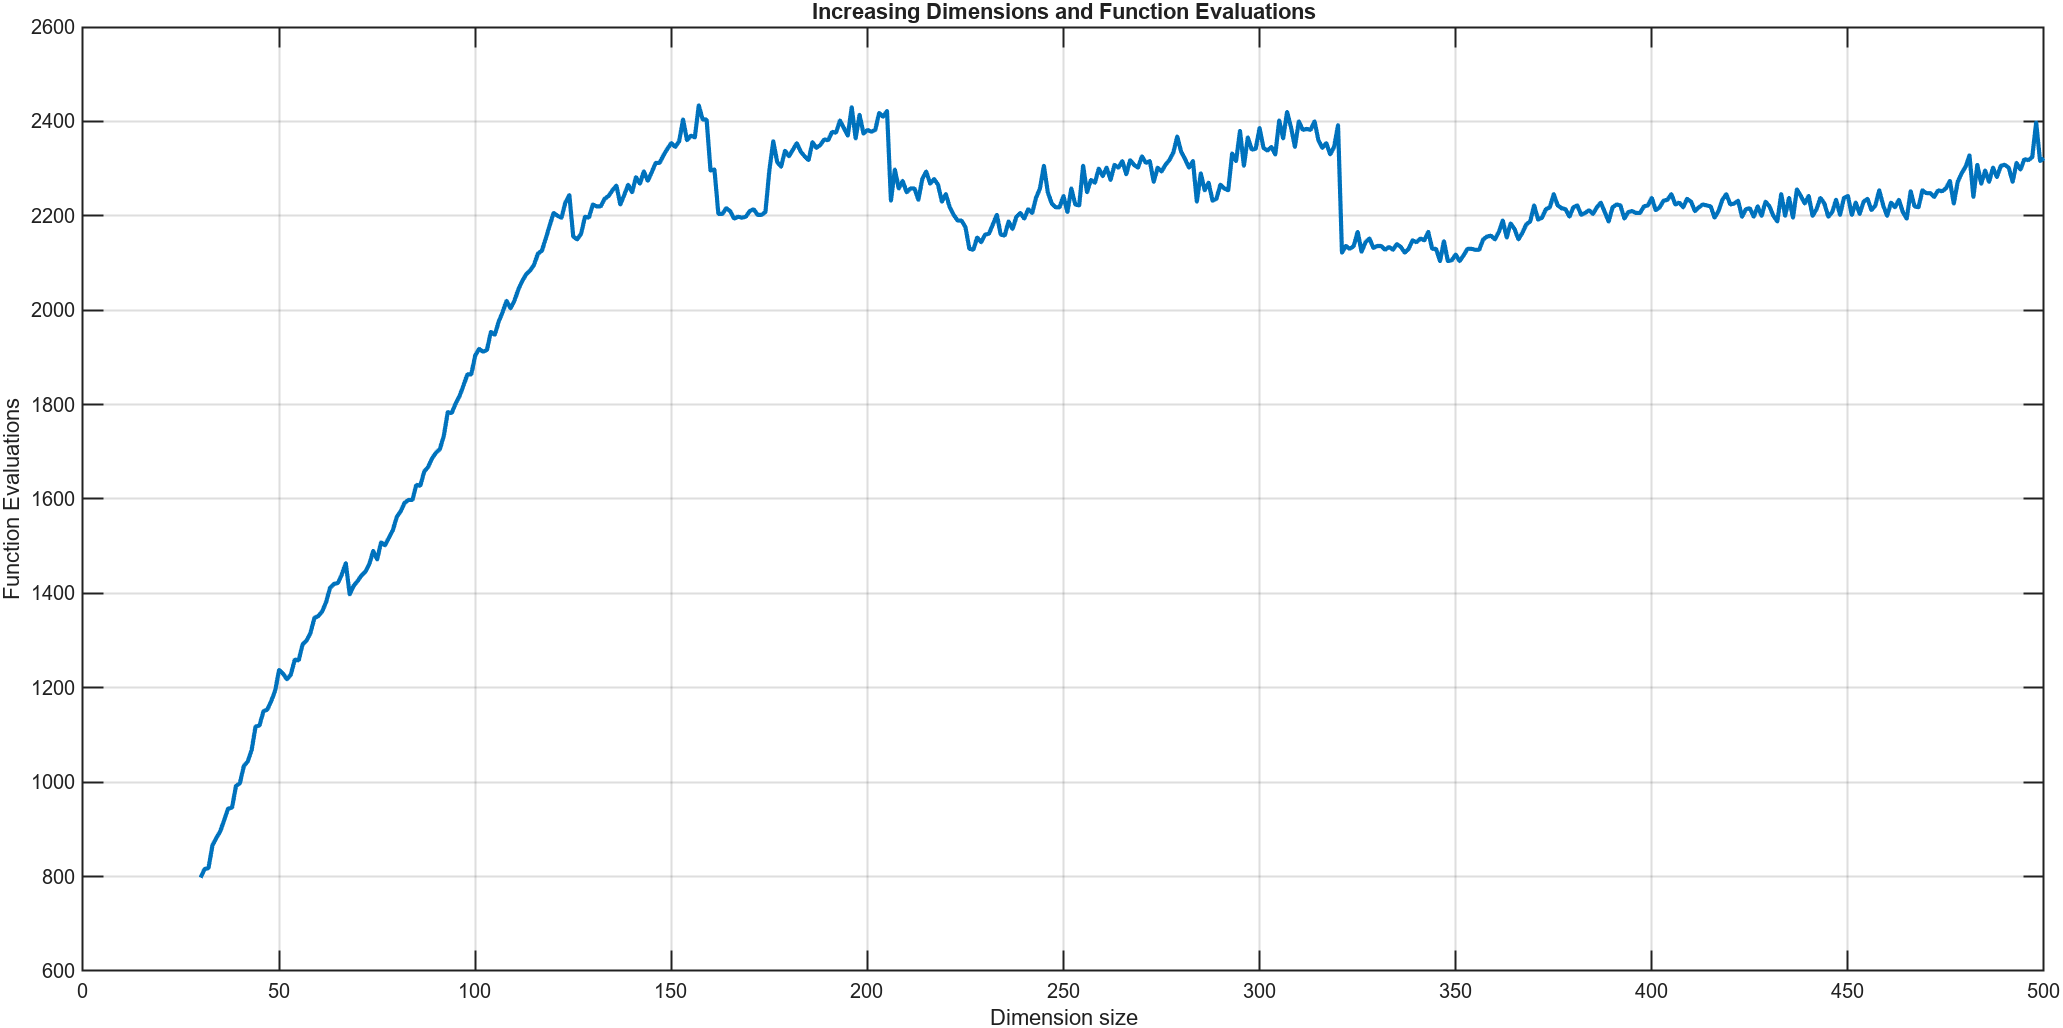
\includegraphics[width=0.8\textwidth]{Plots/inc_dim.png}
    \caption{BFGS function evaluation for increasing dimensions.}
    \label{fig:inc-dim}
\end{figure}

\newpage
\subsection{Problem 4, part b}
Suggest an empirical method to decide whether you observe superlinear convergence and apply it. 
\partbreak
\begin{solution}

    Because we are in a numerical scenario, it isn't feasible to take ratios of increasingly small numbers. I have then two figures to convince us that there is superlinear convergence. Note that, for a general formula to find the power of convergence, we have
    \[q \approx \frac{\log \left( \frac{e_{n+1}}{n}\right)}{\log \left( \frac{e_{n-1}}{e_n}\right)}\]

    We can also just look at the value of the sequence $\norm{x_k - x\star}$, if it converges faster than linear in a log scale, then we can reasonably say we have superlinear convergence. Figure \ref{fig:sup-conv} shows this for the initial dimensions and conditions described above. It \textit{seems} that we have superlinear convergence in this scenario, as this curve decreases faster than linear in the log scale. We also have the $q$ ratio test described above: It's not the most convincing since the plot jumps around too much to determine superlinear convergence $q \in (1, 2)$. This is shown in Figure \ref{fig:sup-conv2}. The value of $q$ usually stays between $-1$ and $2$, which is odd, but is approximately correct. Apologies for the formatting on the second plot, it was a last minute inclusion. 
\end{solution}

\vspace{15mm}
\begin{figure}[!ht]
    \centering
    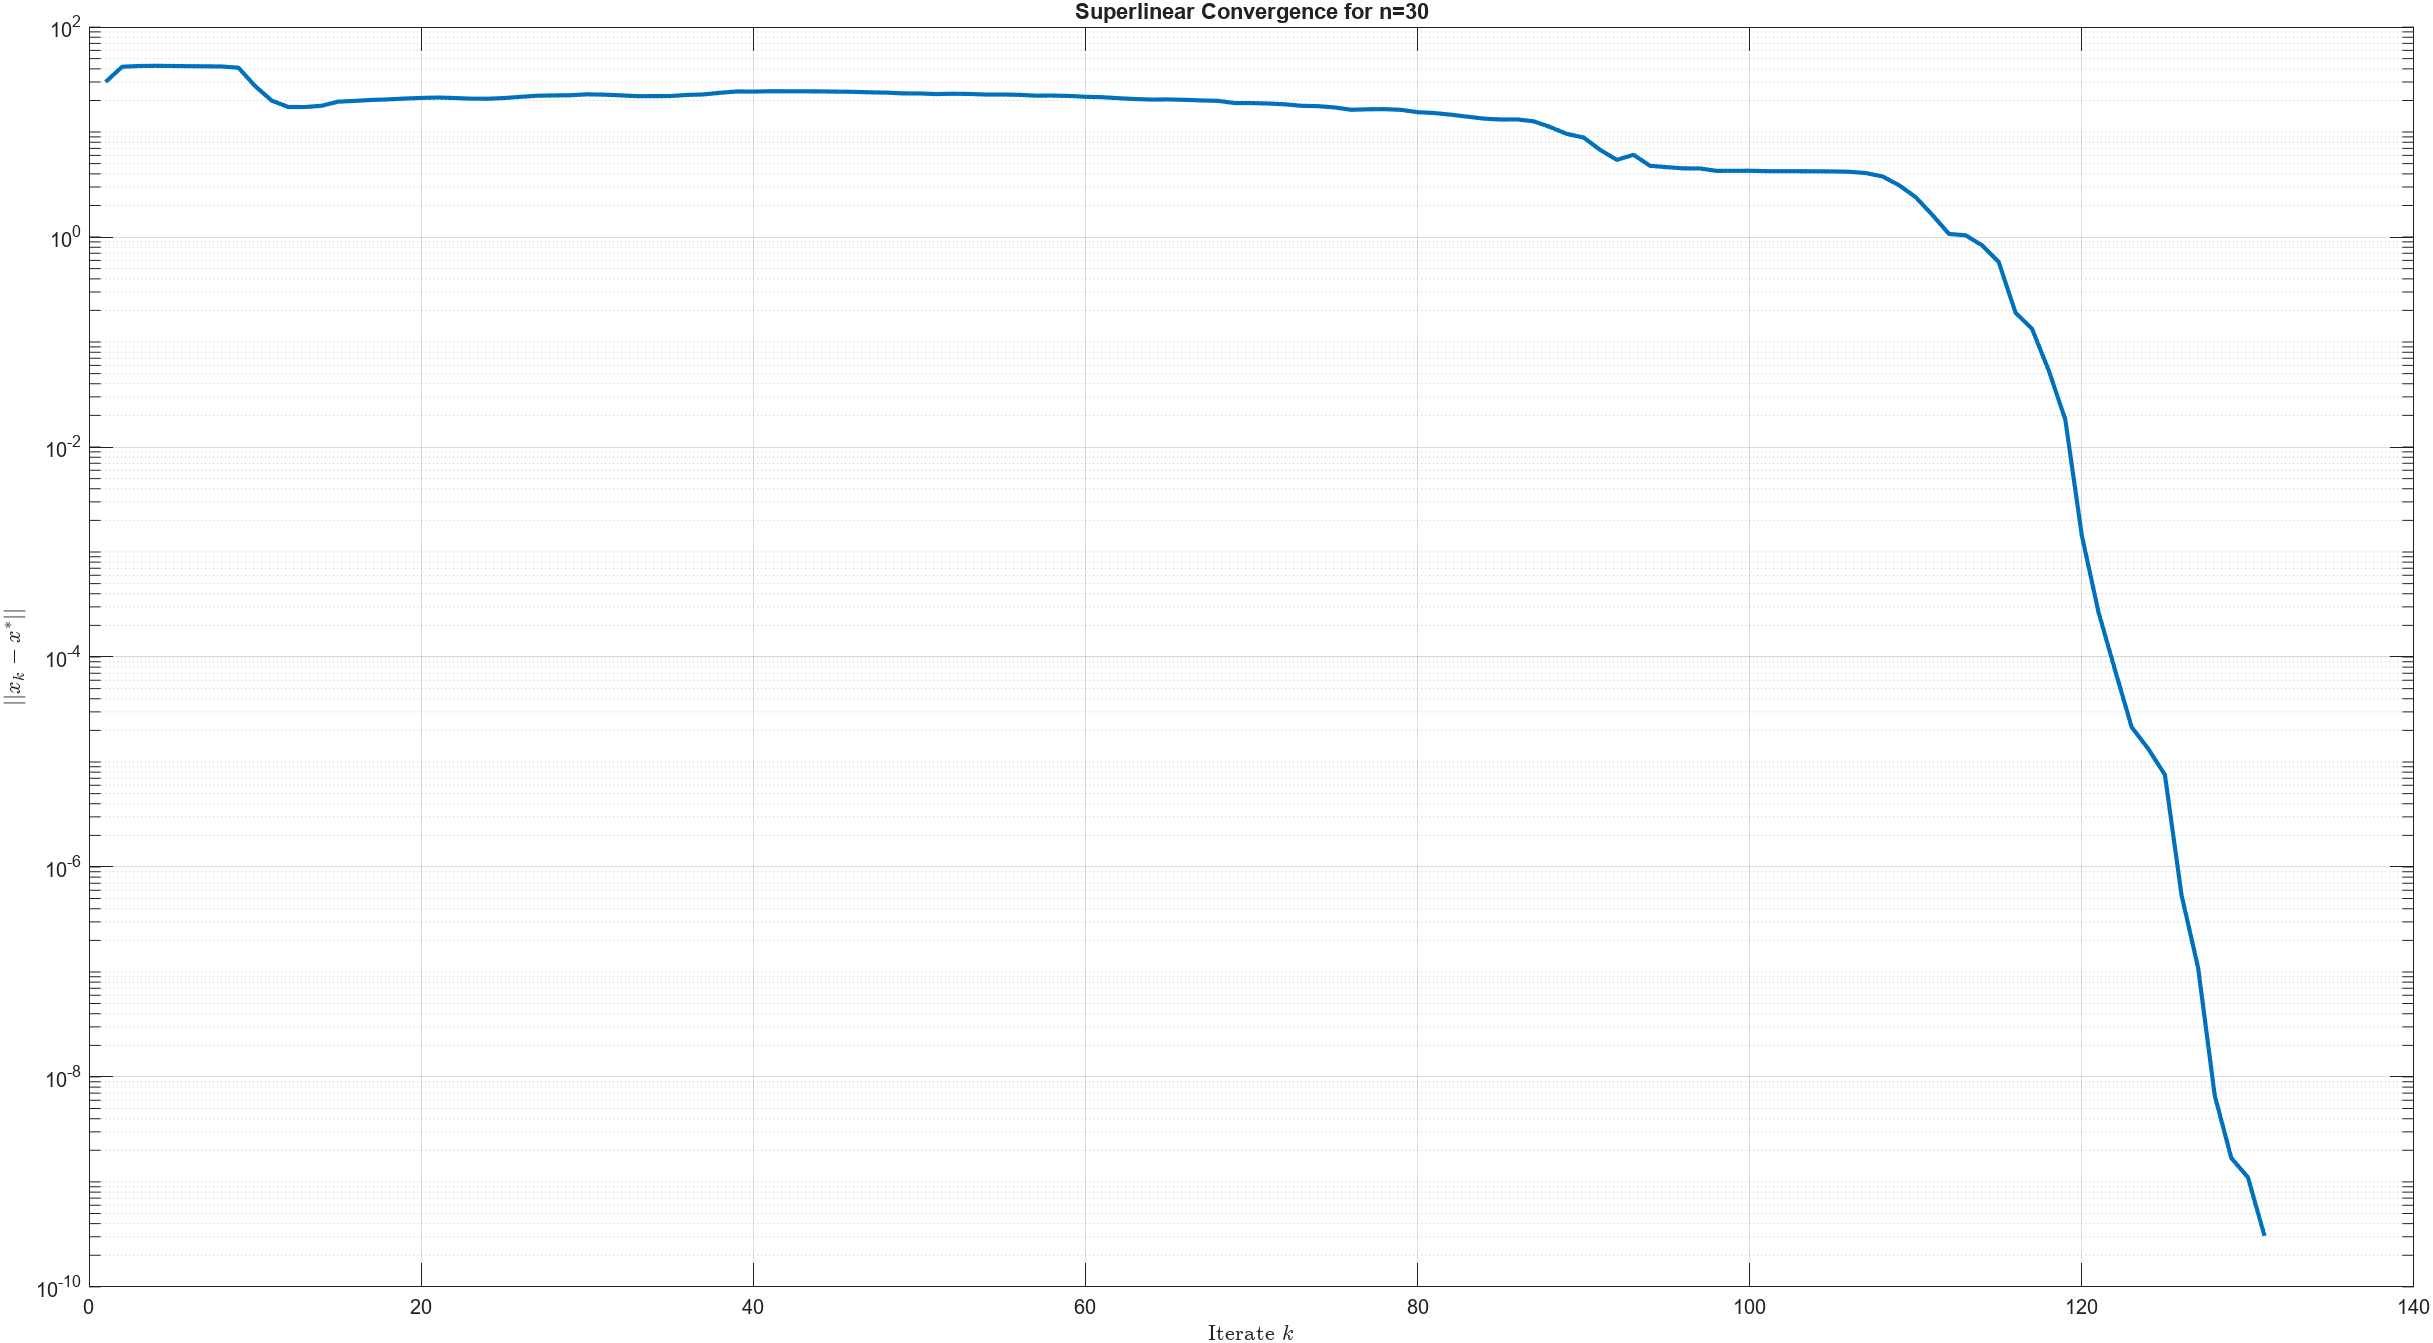
\includegraphics[width=0.8\textwidth]{Plots/sup_conv.png}
    \caption{Value of the sequence of iterates $\norm{x_k - x\star}$.}
    \label{fig:sup-conv}
\end{figure}

\clearpage
\begin{figure}[!h]
    \centering
    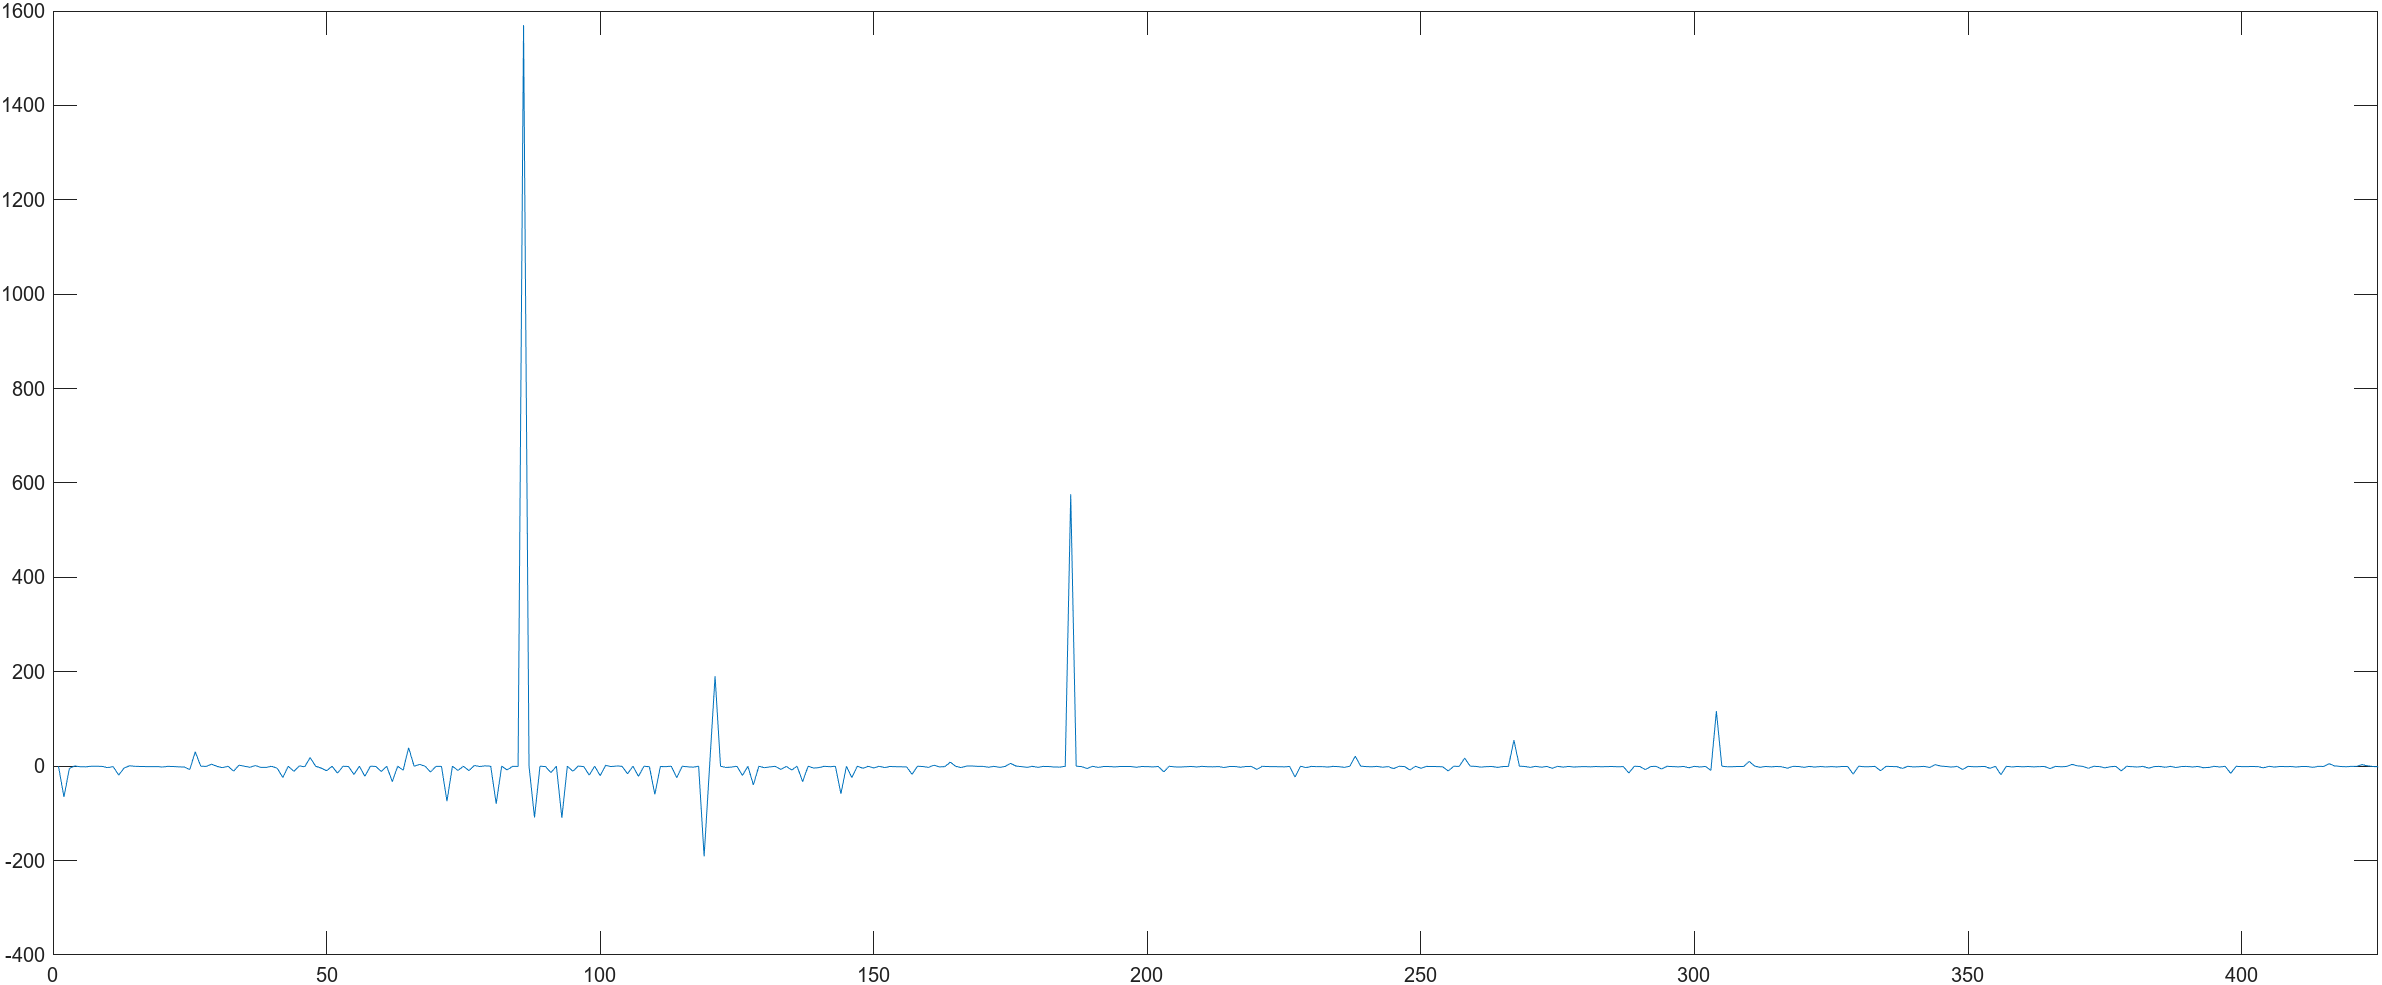
\includegraphics[width = 0.8\textwidth]{Plots/sup_conv2.png}
    \caption{Ratio of convergence.}
    \label{fig:sup-conv2}
\end{figure}
\end{document}